\documentclass{standalone}
\usepackage{tikz}
\usetikzlibrary{arrows.meta, positioning, shapes.geometric}

\begin{document}
    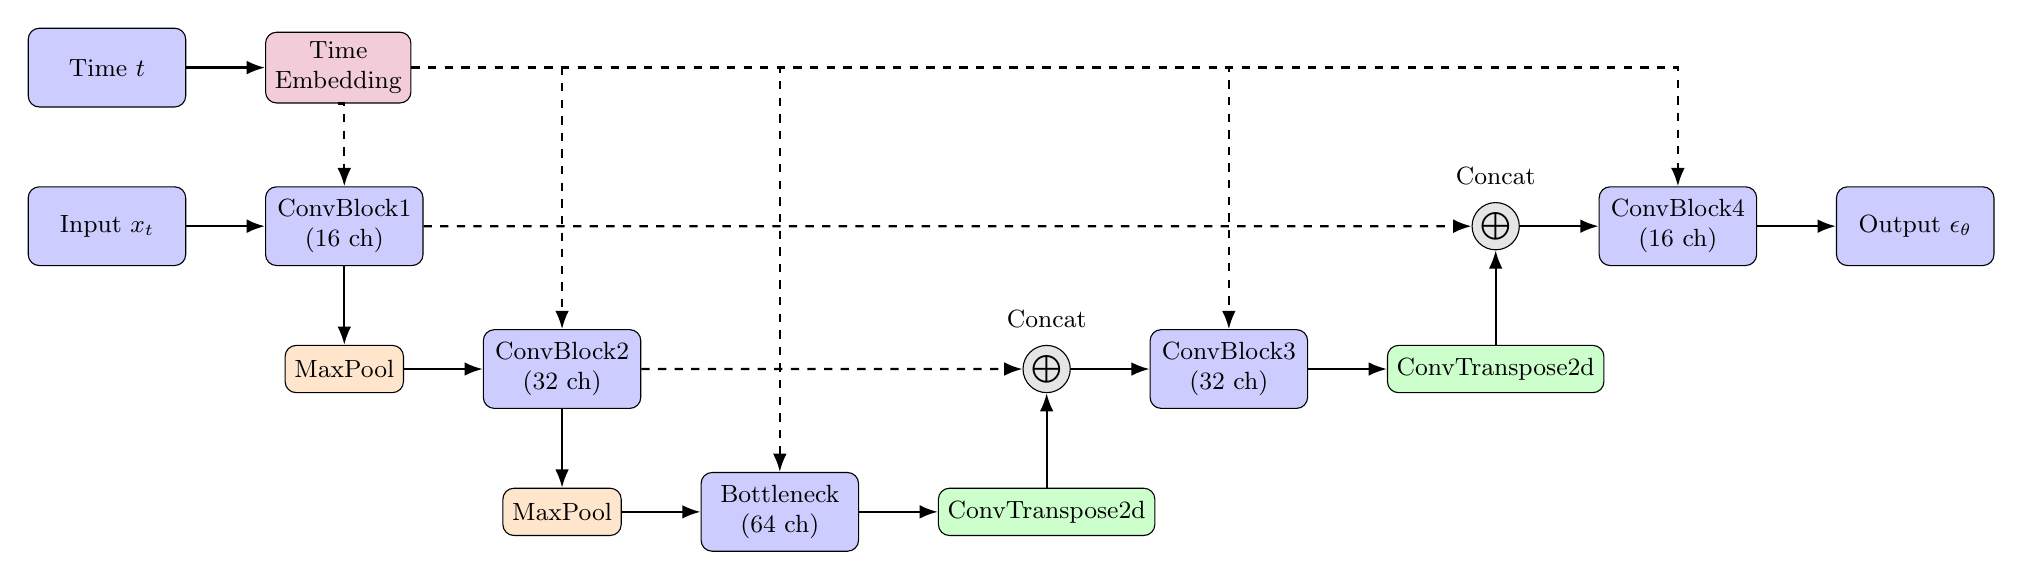
\begin{tikzpicture}[font=\small, node distance=1.5cm]

% Styles
        \tikzstyle{block}=[rectangle, draw, fill=blue!20, rounded corners, minimum height=1cm, minimum width=2cm, align=center]
        \tikzstyle{smallblock}=[rectangle, draw, fill=blue!20, rounded corners, minimum height=0.8cm, minimum width=1.5cm, align=center]
        \tikzstyle{pool}=[rectangle, draw, fill=orange!20, rounded corners, minimum height=0.6cm, minimum width=1.5cm, align=center]
        \tikzstyle{upconv}=[rectangle, draw, fill=green!20, rounded corners, minimum height=0.6cm, minimum width=1.5cm, align=center]
        \tikzstyle{embed}=[rectangle, draw, fill=purple!20, rounded corners, minimum height=0.6cm, minimum width=1.5cm, align=center]
        \tikzstyle{concat}=[circle, draw, fill=gray!20, minimum size=0.6cm, inner sep=0pt, align=center]
        \tikzstyle{arrow}=[-Latex, thick]
        \tikzstyle{skip}=[-Latex, dashed, thick]

% Nodes
% Input
        \node[block] (input) {Input $x_t$};

% Encoder 1
        \node[block, right=1cm of input] (enc1) {ConvBlock1\\(16 ch)};

% Pooling 1
        \node[pool, below=1cm of enc1] (pool1) {MaxPool};

% Encoder 2
        \node[block, right=1cm of pool1] (enc2) {ConvBlock2\\(32 ch)};

% Pooling 2
        \node[pool, below=1cm of enc2] (pool2) {MaxPool};

% Bottleneck
        \node[block, right=1cm of pool2] (bottleneck) {Bottleneck\\(64 ch)};

% Upconv 2
        \node[upconv, right=1cm of bottleneck] (upconv2) {ConvTranspose2d};

% Concatenate 1
        \node[concat, above=1.2cm of upconv2] (concat1) {$\bigoplus$};

% Decoder 2
        \node[block, right=1cm of concat1] (dec2) {ConvBlock3\\(32 ch)};

% Upconv 1
        \node[upconv, right=1cm of dec2] (upconv1) {ConvTranspose2d};

% Concatenate 2
        \node[concat, above=1.2cm of upconv1] (concat2) {$\bigoplus$};

% Decoder 1
        \node[block, right=1cm of concat2] (dec1) {ConvBlock4\\(16 ch)};

% Output
        \node[block, right=1cm of dec1] (output) {Output $\epsilon_{\theta}$};

% Time input
        \node[block, above=1cm of input] (time) {Time $t$};

% Embedding
        \node[embed, right=1cm of time] (embedding) {Time\\Embedding};

% Connections
% Forward Path
        \draw[arrow] (input) -- (enc1);
        \draw[arrow] (time) -- (embedding);
        \draw[arrow] (enc1) -- (pool1);
        \draw[arrow] (pool1) -- (enc2);
        \draw[arrow] (enc2) -- (pool2);
        \draw[arrow] (pool2) -- (bottleneck);

        \draw[arrow] (bottleneck) -- (upconv2);
        \draw[arrow] (upconv2) -- (concat1);
        \draw[arrow] (concat1) -- (dec2);
        \draw[arrow] (dec2) -- (upconv1);
        \draw[arrow] (upconv1) -- (concat2);
        \draw[arrow] (concat2) -- (dec1);
        \draw[arrow] (dec1) -- (output);

% Skip Connections
%        \draw[skip] (enc2.east) -| ([xshift=1cm]enc2.east) |- (concat1.west);
        \draw[skip] (enc2) -- (concat1);
        \draw[skip] (enc1) -- (concat2);

% Embedding Connections
        \draw[arrow, dashed] (embedding.south) -- ++(0,0) -| (enc1.north);
        \draw[arrow, dashed] (embedding.east) -- ++(0,0) -| (enc2.north);
        \draw[arrow, dashed] (embedding.east) -- ++(0,0) -| (bottleneck.north);
        \draw[arrow, dashed] (embedding.east) -- ++(0,0) -| (dec2.north);
        \draw[arrow, dashed] (embedding.east) -- ++(0,0) -| (dec1.north);

% Labels
        \node[above=0.1cm] at (concat1.north) {Concat};
        \node[above=0.1cm] at (concat2.north) {Concat};

    \end{tikzpicture}
\end{document}
